\chapter{Écoles de devoirs}
\section{Gestion de vos écoles de devoirs}
Vous pouvez accéder à la gestion de vos EDD, en développant le volet \ovalbox{Écoles de devoirs}, puis en cliquant sur l'entrée \ovalbox{Lieux}. Vous pouvez également utiliser le raccourci "consulter les Écoles de devoirs" de la page d'accueil.

La liste de vos écoles de devoirs reconnues auprès de l'ONE apparaît. En cliquant sur la ligne d'une de vos écoles de devoirs, vous accéderez à sa gestion. Plusieurs onglets vous seront disponibles. 
\vspace{1cm}

\centerline{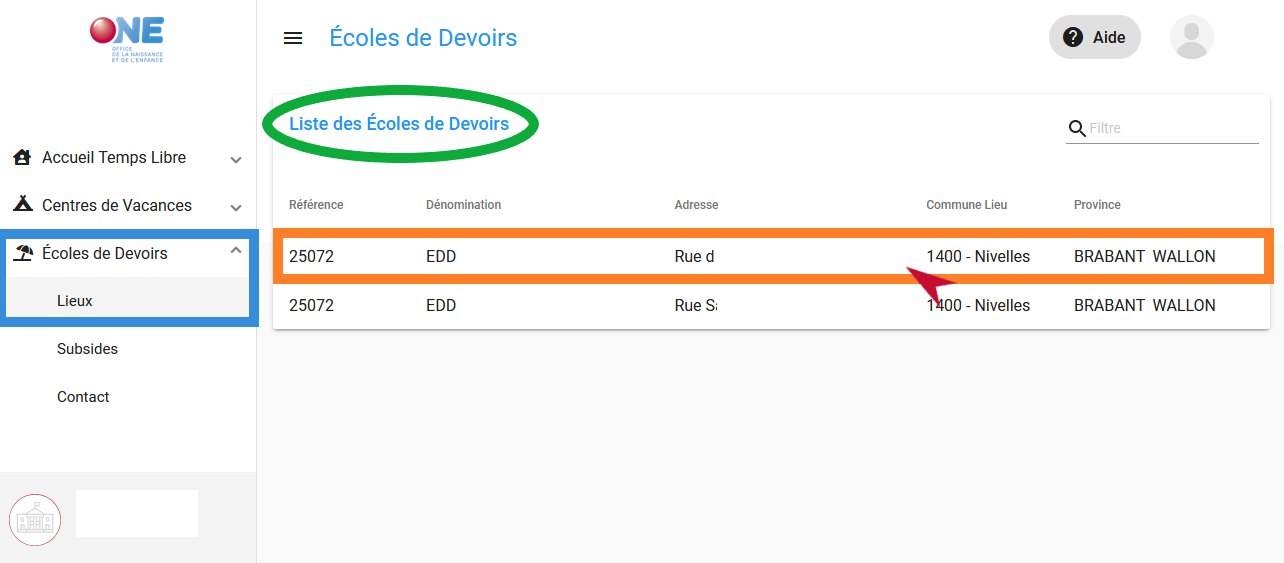
\includegraphics[width=13cm]{Images/edd/edd-lieu.png}}


\subsection{L'onglet lieu: informations de base de l'EDD}
\begin{itemize}
    \item \textbf{Lieu}: vérifiez l'adresse du lieu. Si les données ne sont pas correctes, prenez contact avec votre conseillère EDD. 
    \item \textbf{Caractéristiques de l'EDD}: encodez la participation financière demandée aux parents.
    \item \textbf{Personne de contact de l'EDD}: il est possible de mentionner une personne de contact spécifique à l'EDD (un animateur référent, le coordinateur,  un bénévole administratif, etc.).
\end{itemize}

\subsection{L'onglet horaire: informations sur les heures d'ouverture en période scolaire}    
Encodez les horaires de l'année en cours. Lors de l'introduction de la demande de subvention, il faudra renseigner les horaires de l'année suivante.

Cliquez sur le petit crayon de modification pour encoder et mettre à jour. Ensuite, complétez les heures (en bleu). Vous pouvez également ajouter des commentaires si nécessaire (en vert). N'oubliez pas ensuite de \ovalbox{valider} vos modifications. 

\begin{info}
Si vous encodez deux années consécutivement, validez l'encodage de la première année avant de passer à la suivante.
\end{info}
 

\begin{figure}[htbp]
    \centering
    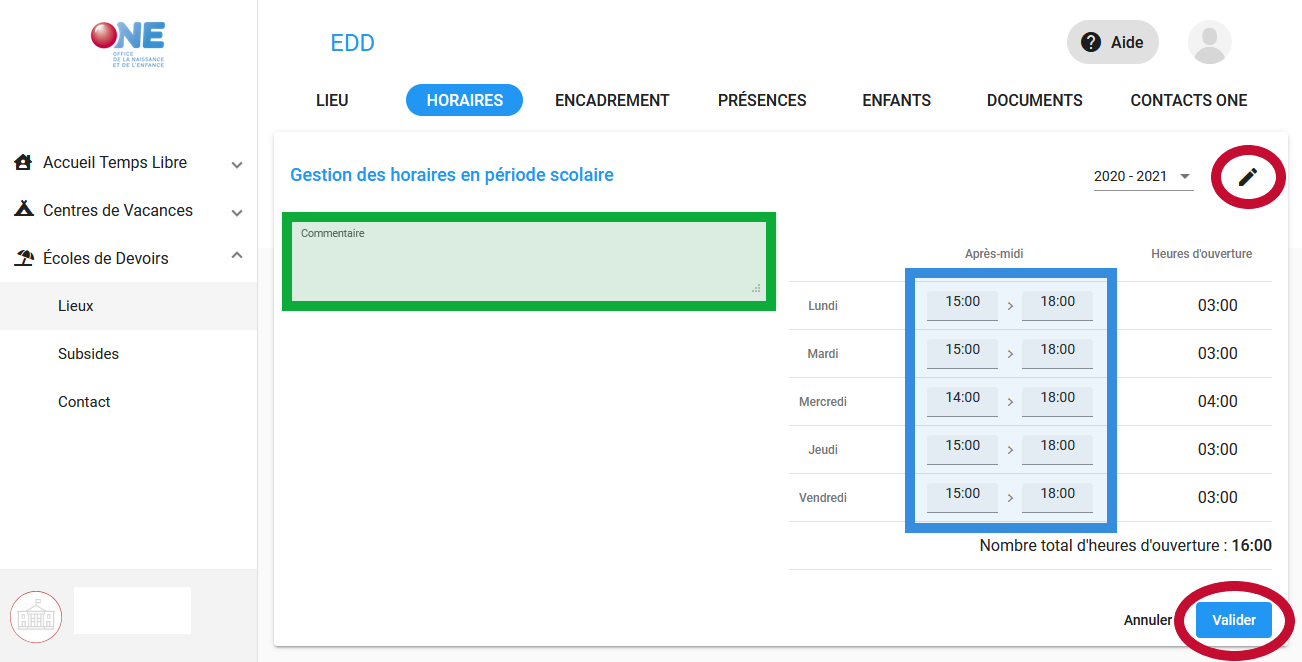
\includegraphics[width=14cm]{Images/edd/edd-horaires.png}
    \caption{Onglet horaire: les heures d'ouverture en période de scolaire de votre école de devoirs.}
    \label{fig:edd_horaires}
\end{figure}

    
\subsection{L'onglet encadrement: liste des membres de l'équipe}

\begin{figure}[htbp]
    \centering
    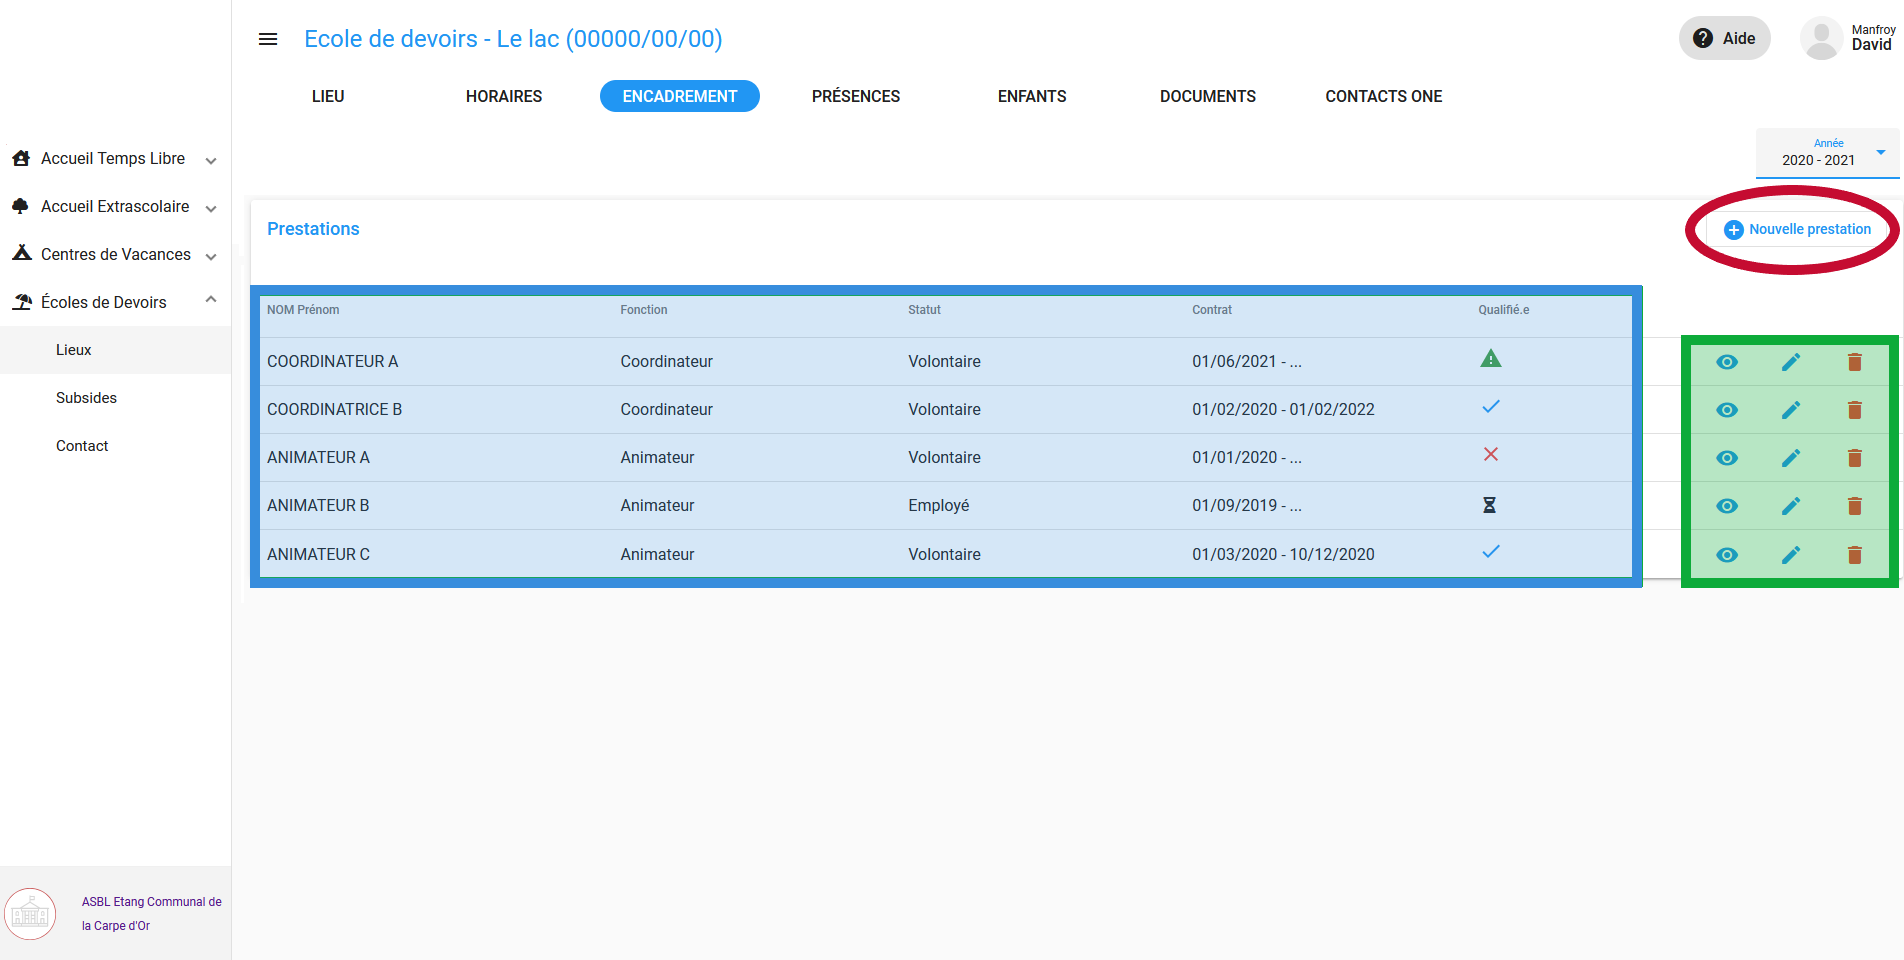
\includegraphics[width=15cm]{Images/edd/encadrement.png}
    \caption{Onglet encadrement: liste du personnel qui preste pour l'école de devoirs.}
    \label{fig:edd_encadrement}
\end{figure}


Cet onglet reprend le personnel d'encadrement qui preste pour votre école de devoirs (fig. \ref{fig:edd_encadrement}. Vous renseignerez les coordinateurs et les animateurs qui ont animé les enfants (en \textcolor{bleu}{bleu}). Pour chacun d'eux, vous pourrez renseigner leur fonction (coordination ou animation), leur statut (employé, volontaire ou stagiaire), leur contrat/convention et les qualifications pour leur fonction (qualifié ou non qualifié).

\subsubsection{Prestation, qualification ou suppression}
Quelques boutons d'action sont disponibles (en \textcolor{vert}{vert} dans la fig. \ref{fig:edd_encadrement}):


\begin{itemize}
    \item Les \textbf{qualifications} peuvent être renseignées en cliquant sur l'icône 
\includegraphics[width=0.3cm]{Images/icon/button_dmd_qualif.png}.
    \item Les informations de \textbf{prestation} (fonction et statut) sont modifiables en cliquant sur 
\includegraphics[width=0.3cm]{Images/icon/button_modif.png}.
    \item Vous avez également la possibilité de \textbf{supprimer la prestation} en cliquant sur 
\includegraphics[width=0.3cm]{Images/icon/button_poubelle.png}. Celle-ci n'apparaîtra alors plus dans le personnel de votre activité et les données de présences seront supprimées (onglet présences).
\end{itemize} 




\subsubsection{Ajouter un membre de l'équipe d'encadrement}
Cliquez sur \ovalbox{Ajouter une prestation} en haut à droite. Dans l'encadré \fbox{\textbf{Nouvelle prestation}} (fig. \ref{fig:edd_new_prestation}), vous serez invité à ajouter l'encadrant, à indiquer le contexte de sa prestation (contrat de travail, étudiant, stage ou convention de volontariat par exemple), sa fonction et son statut. 

\begin{figure}[htbp]
    \centering
    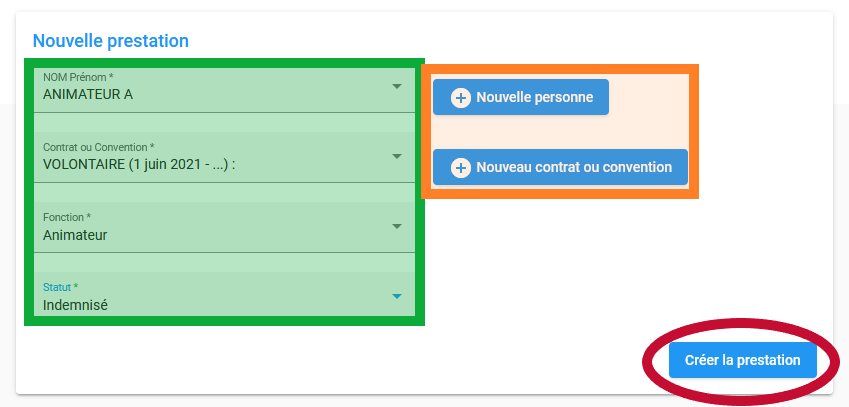
\includegraphics[width=10cm]{Images/edd/new_prestation.png}
    \caption{Cadre Nouvelle prestation}
    \label{fig:edd_new_prestation}
\end{figure}


\begin{enumerate}
    \item En cliquant sur "\textbf{prénom nom}*", vous aurez accès à la liste des personnes qui ont déjà travaillé pour votre pouvoir organisateur dans une école de devoirs;  sélectionnez ensuite la personne dans la liste. Si par contre, la personne ne figure pas dans la liste, cliquez sur \ovalbox{Ajouter une personne}. Vous serez alors dirigé vers "Mon Équipe" pour créer la personne (NISS + Prénom + Nom) et son lien contractuel avec votre Pouvoir organisateur. 
    \begin{conseil}
     Pour vous aider, suivez le point \ref{team_add_person} "Ajouter une personne dans Mon Équipe".
    \end{conseil}
    
    \item En cliquant sur "\textbf{Contrat et convention}", la liste vous donnera l'ensemble des liens (contractuels ou conventionnels) que la personne entretient avec votre pouvoir organisateur. La liste ne vous affichera que les contrats/conventions qui sont actifs. 
    \begin{conseil}
     Pour vous aider, suivez le point \ref{team_add_contract} "Ajouter un contrat/un lien".
    \end{conseil}    

    
    \item Ajoutez la \textbf{fonction}: animateur ou coordinateur. 
        \begin{attention}
         Si la personne anime un jour et coordonne l'école de devoirs un autre jour, il sera nécessaire de l'encoder deux fois. La personne ne pourra pas détenir les deux fonctions pour un même jour (il anime ou il coordonne, mais pas les deux au niveau du calcul de la subvention), mais il peut animer un jour et coordonner un autre jour.
        \end{attention}
    \item Indiquez le \textbf{statut de la personne}: employé ou volontaire. Ces champs seront pré-remplis en fonction du point 2 (contrat et convention), mais pourront être modifiés. 
    \item Cliquez enfin sur \ovalbox{Créer la prestation}. La personne sera alors ajoutée à la liste des encadrants de votre activité.
\end{enumerate}

\vspace*{4mm}
\begin{tcolorbox}[title=La personne ou le contrat/convention de celle-ci n'apparaît pas dans la liste]
La liste reprend les informations encodées dans "Mon Équipe":
\begin{itemize}
    \item \textbf{Pour les personnes}: elles doivent avoir été ajoutées dans Mon Équipe. Elles doivent en outre avoir un contrat en lien avec le secteur Écoles de devoirs encodées dans mon Équipe.
    \item \textbf{Pour les contrats/conventions}: la liste ne reprendra que les contrats/conventions actifs.
\end{itemize}

Si les éléments que vous recherchez ne sont pas présents, cliquez sur \ovalbox{Créer une personne} ou \ovalbox{Créer un nouveau contrat/convention}. Suivez le point \ref{team_add_person} "Ajouter une personne dans Mon Équipe" et le point \ref{team_add_contract} "Ajouter un contrat/un lien" (chapitre \ref{chap:team} de ce Guide). 

\textbf{Remarque}: il sera peut être nécessaire non pas de créer un contrat (au risque d'avoir plusieurs même contrat encodée), mais d'adapter un contrat déjà existant dans Mon Équipe. Pour cela, développez Accueil Temps Libre, cliquez sur Mon Équipe. Rendez-vous ensuite dans la fiche de la personne pour modifier son ou ses contrats.  

\end{tcolorbox}

\subsubsection{Consulter les qualifications de la personne}

Dans l'encadré \textcolor{vert}{vert} de la fig. \ref{fig:cdv_encadrement}, vous pouvez voir les qualifications de la personne connues par l'ONE:

\begin{itemize}
    \item [$\bullet$]\textbf{\textcolor{bleu}{V}}: la personne est qualifiée pour exercer sa fonction d'animation ou de coordination. 
    \item [$\bullet$]\textbf{\textcolor{rouge}{X}}: la personne n'est pas qualifiée pour exercer sa fonction d'animation ou de coordination. 
    \item [$\bullet$]
\includegraphics[width=0.3cm]{Images/icon/icon_sablier.png}: une demande de qualification est en cours d'analyse auprès de l'ONE. 
    \item [$\bullet$]
\includegraphics[width=0.4cm]{Images/icon/icon_attention.png}: la personne a obtenu sa qualification durant l'année en cours. En fonction de la date d'octroi de la qualification, le calcul de subventionnement peut être impacté. En effet, la personne est considérée comme non qualifiée avant cette date. 
\end{itemize}
\vspace*{3mm}

\begin{tcolorbox}[title=Les trois possibilités de qualification EDD]
Pour le secteur Écoles de devoirs, la personne peut: 

\begin{enumerate}
    \item Être en possession du \textbf{brevet écoles de devoirs} délivré par La Fédération des Ecoles de devoirs;
    \item Posséder un CESS à orientation sociale ou pédagogique ou un diplôme de l'enseignement supérieur (type court minimum).  
    \item Être en possession d'une \textbf{équivalence au brevet}.
\end{enumerate}
Pour faire reconnaître une qualification, il faut envoyer une demande de qualification depuis la fiche "Mon Équipe" de la personne. 
\end{tcolorbox}

\subsubsection{Envoyer une demande de qualifications}
\begin{itemize}
    \item Cliquez sur 
\includegraphics[width=0.3cm]{Images/icon/button_dmd_qualif.png}. Vous pourrez alors renseigner les preuves de qualification de la personne.
        \begin{conseil}
        Suivez le point \ref{sec:qualif_person} de ce Guide pour faire une demande de qualification (Mon Équipe). 
        \end{conseil}
    \item Une fois la demande de qualification envoyée dans "Mon Equipe", vous pourrez revenir à la gestion de vos encadrants en cliquant sur le petit encadré jaune "Retourner vers la liste des prestations" situé en bas à droite de votre écran.
\end{itemize}

\subsection{L'onglet présences: encodage des présences enfants et encadrants}

Les cases sont grisées en fonction des heures d'ouverture renseignées dans l'onglet \ovalbox{horaire}. Il est néanmoins possible d'encoder des présences pour les jours d'ouverture ponctuels. Sélectionnez d'abord le mois pour lequel vous souhaitez rentrer les présences. Pour les enfants, encodez pour chaque jour le nombre d'enfants accueillis (en bleu). Pour les membres de l'équipe, cliquez sur la case du jour de présence pour confirmer la présence de l'encadrant (en vert). 
\begin{info}
Les données sont enregistrées automatiquement. 
\end{info}

\vspace{1cm}

\centerline{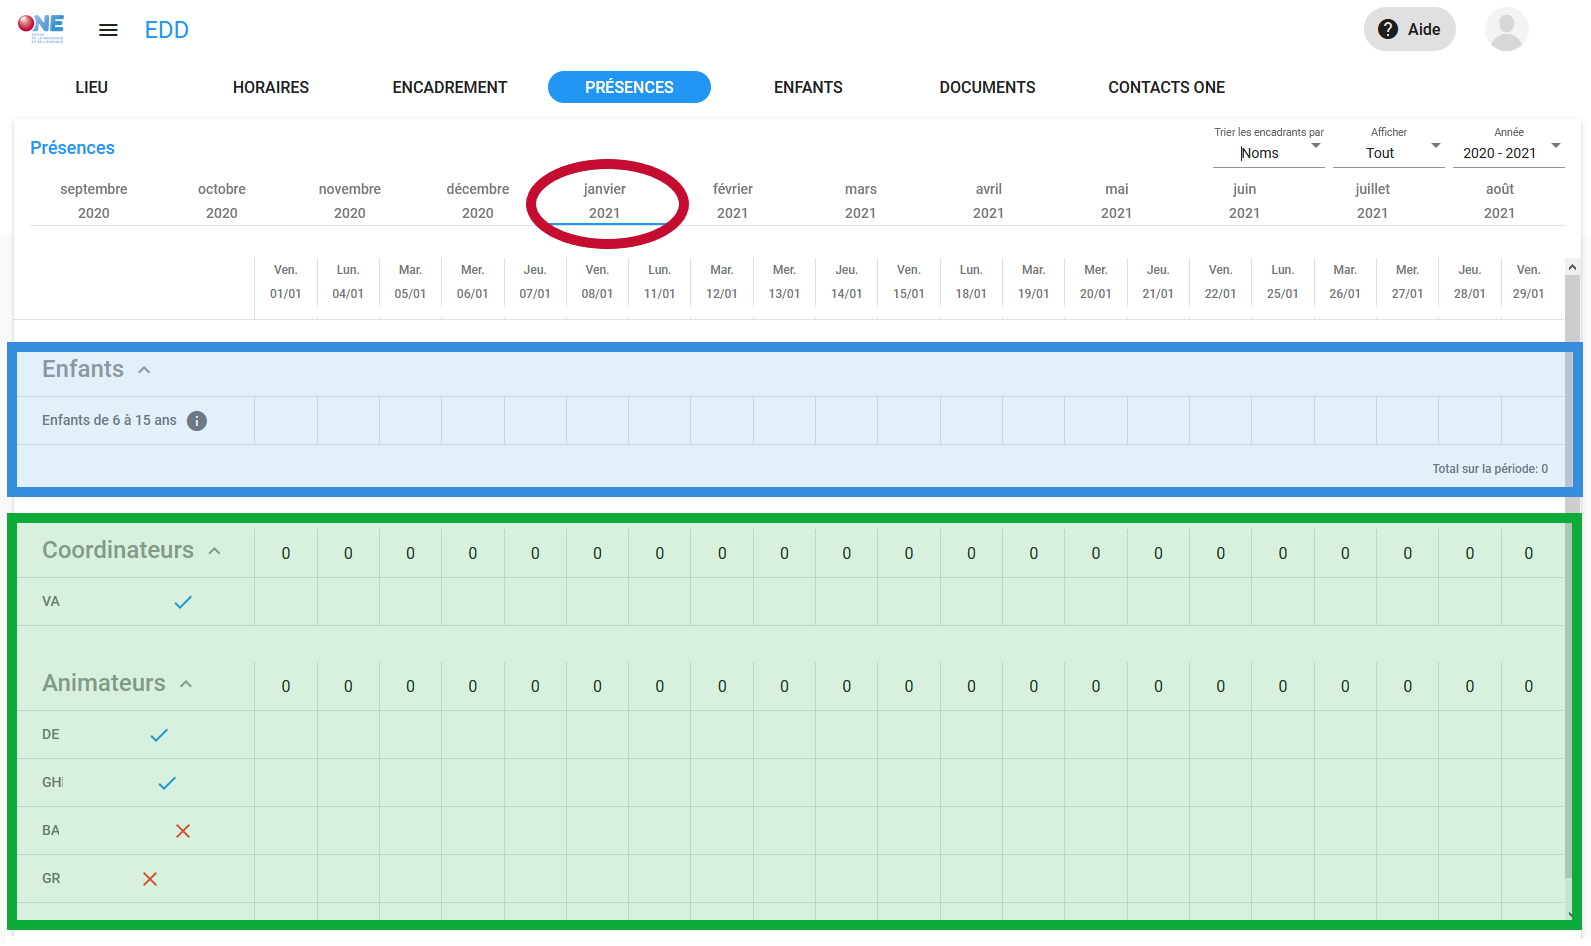
\includegraphics[width=16cm]{Images/edd/edd-presences.png}}

\subsection {L'onglet enfants: liste des enfants}

Dans cet onglet, vous êtes invité à charger la liste des enfants accueillis l’année précédente et à compléter les informations reprises dans la case « résumé ».
\begin{info}
Un canevas de liste nominative est à votre disposition en haut de l’onglet mais vous pouvez télécharger votre propre liste nominative reprenant les informations du canevas.
\end{info}


\section{Demander des subsides pour vos écoles de devoirs}

\begin{enumerate}
    \item \textbf{Entrée \ovalbox{Subsides}}: accédez à la demande de subvention pour chacune de vos EDD en cliquant sur l'onglet "Subsides"
    \item Vérification des données: assurez‐vous d’avoir bien encodé et chargé les données reprises dans cette checklist. Le lien pour accéder au rapport d’activité (RA) en ligne est envoyé chaque année par mail, dans le courant du mois de juin, par le Service EDD.

    \item \textbf{Choix du type de demande}: sélectionnez le type de demande pour chacune de vos EDD:
        \begin{itemize}
            \item Liquidation et subvention
            \item Liquidation uniquement
            \item Subvention = nouvelle demande de subvention
        \end{itemize}
En cochant la case, vous engagez la responsabilité du Pouvoir organisateur quant à la l'exactitude des informations.

\item \textbf{Accueil vacances d’automne et de détente}:veuillez cocher la case « Accueil prévu en automne et en détente » pour chaque EDD qui organiserait des journées d’activités lors de ces vacances (min. 6h/jour). Si l’organisation d’activités est encore incertaine, nous vous conseillons de cocher la case par défaut. 


%\centerline{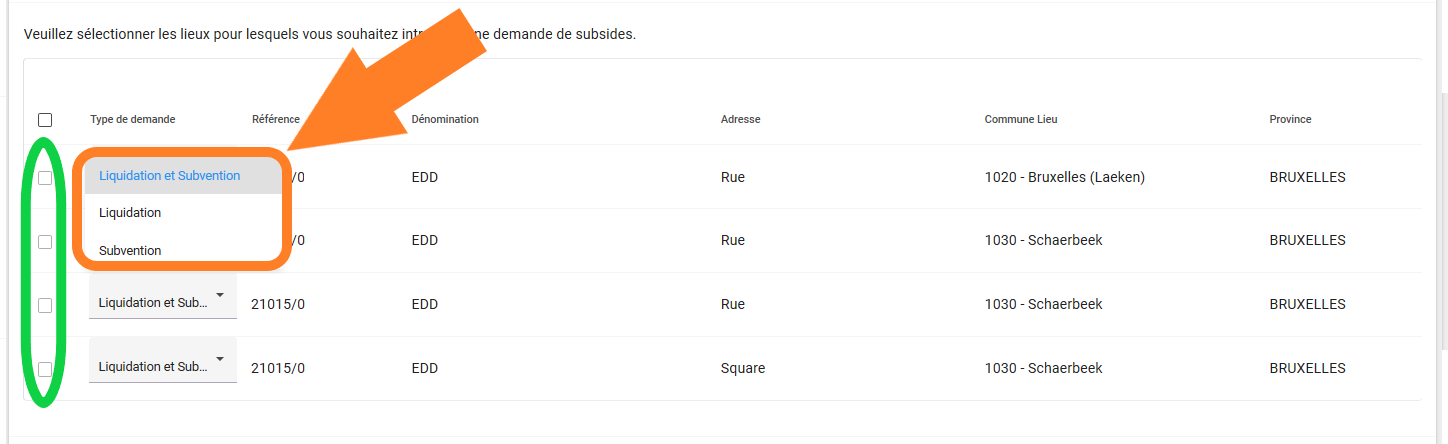
\includegraphics[width=12cm]{Images/edd/edd-choix-ds.png}}

    \item \textbf{Envoi de la demande}: cliquez sur "introduire la demande" pour l'envoyer. Après cela, il n'est plus possible d'y apporter des modifications. S'il y a des compléments à fournir, prenez contact avec votre conseillère. 
    \begin{remarque}
    Si vous avez plusieurs lieux EDD , la demande doit être introduite simultanément pour l'ensemble de vos EDD. Dès lors, assurez-vous que toutes les informations requises pour chacune d'entre elles sont complètes.
    \end{remarque}
 
    \item \textbf{Traitement de la demande}: une fois la demande envoyée, la date d'envoi apparaît et elle est prête à être analysée par votre conseillère. Celle-ci reviendra vers vous s'il y a des compléments à transmettre.

    
\end{enumerate}

\begin{attention}\normalfont
Pour rappel, la demande de subvention doit être introduite pour le \textcolor{rouge}{\textbf{30 septembre au plus tard}}.
\end{attention}

\section{Consulter le résultat de calcul de votre subvention}
Dans le volet de navigation à gauche, en cliquant sur \ovalbox{Subsides}, vous pourrez consulter les demandes de subsides que vous avez introduites via l'onglet \ovalbox{demande}.

\vspace{4mm}
\centerline{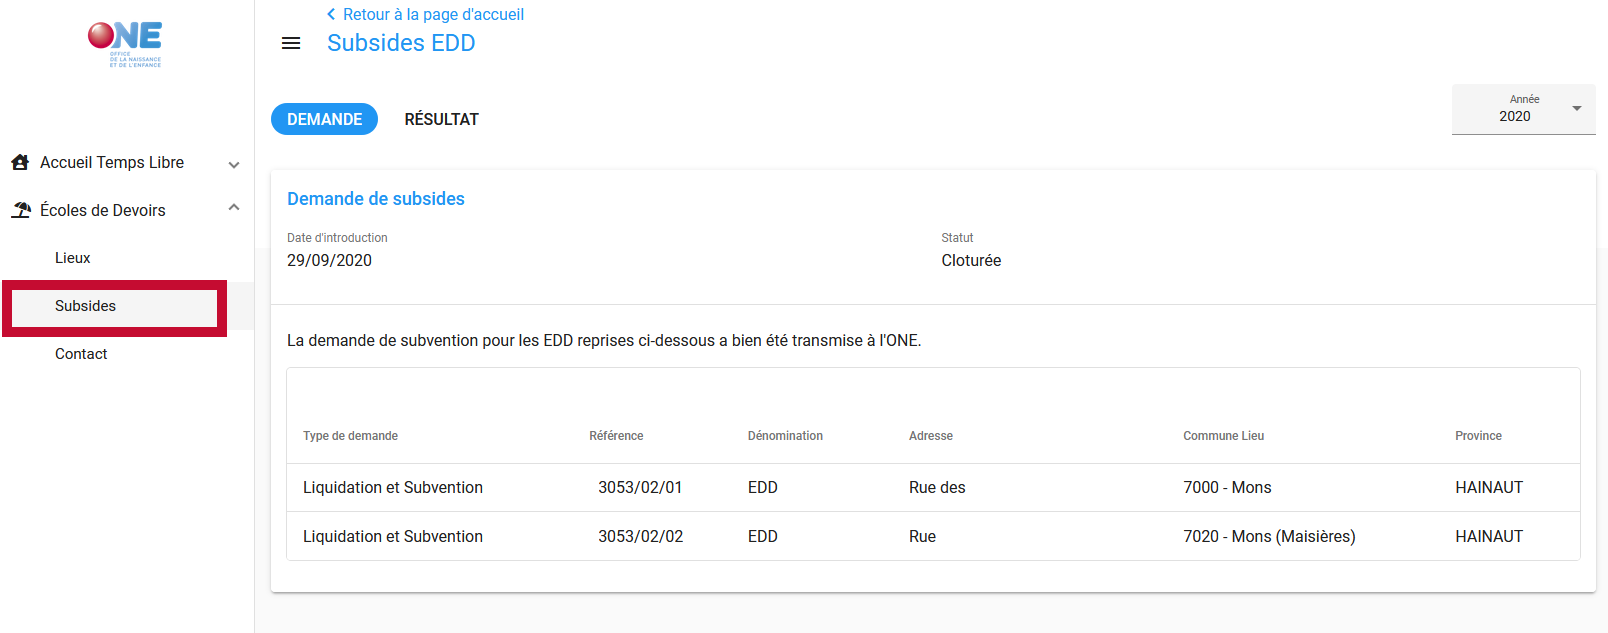
\includegraphics[width=15cm]{Images/edd/edd-subsides.png}}

Le solde est calculé suite à l’analyse de votre demande de liquidation. Lorsque la subvention est calculée par l’ONE, vous pourrez consulter le  montant total de la subvention théorique pour l’année en cours, ainsi que le montant de l’avance (70\%) et le montant du solde théorique (30\%) via l'onglet \ovalbox{résultat}. 

\vspace{4mm}
\centerline{\includegraphics[width=15cm]{Images/edd/edd-résultats.png}}

